% Součást skript na Datové struktury. Viz main.tex
\markright{$ $Id$ $}

\chapter{Hašování II}

% --------------------------------------------------------------------------
\section{Univerzální hašování}

Idea univerzálního hašovaní má odstranit požadavek na rovnoměrné 
rozložení vstupních dat. Tento požadavek chceme nahradit tím, že 
budeme mít soubor $H$ hašovacích funkcí do tabulky velikosti $m$ takový,
že pro každou podmnožinu $S$ univerza $U$ je pravděpodobnost, že funkce z 
$H$ se chová dobře, hodně velká (tj. je jen málo kolizí). V tomto případě, 
když vybereme $h$ z $H$ náhodně s rovnoměrným rozložením, pak pro každou 
podmnožinu $S\subseteq U$ takovou, že $|S|\leq m$, bude očekávaný čas 
(počítaný přes všechny funkce z $H$) konstantní. Rozdíl proti tradičnímu 
hašovaní je, že předpoklad rovnoměrného výběru hašovací funkce z množiny 
$H$ můžeme zajistit (nebo se k splnění tohoto požadavku přiblížit), ale 
výběr vstupních dat ovlivnit nemůžeme. Nyní tuto ideu zformalizujeme. 
\mnote{zajímá nás jednak $c$, jednak velikost systému (tj. počet funkcí v
systému)}

\begin{defn}
\label{c-us}
Třída hašovacích funkcí 
\( H \subseteq \{h | h: \intrange{0}{N-1} \rightarrow \intrange{0}{m-1}\} \)
je \emph{c-univerzální} systém, kde $c\in\mathbb{R}^+$, jestliže 
\begin{equation*}
\forall x\neq y\in \intrange{0}{N-1} :
\left |\{h\in H : h(x)=h(y)\}\right| \leq c\frac{|H|}{m}, 
\end{equation*}
\end{defn}

%Dolní mez pro $c$, dk na cvičení.
% rádi bychom \( c \) co nejmenší, ale dá se dokázat,
% že neexistují \( c \)-univerzální třídy pro
% \( c<1-\frac{m}{N} \).

% ..........................................................................

\noindent
Nejprve ukážeme, že $c$-univerzální systémy existují:

\begin{theorem}
Předpokládejme, že $U = \intrange{0}{N-1}$, kde $N$ je prvočíslo.
Definujme 
\[ H=\{h_{ab}:h_{ab}(x)=((ax+b)\bmod N)\bmod m;
\ a,b\in \intrange{0}{N-1}\} \]

Potom $H$ je \( c \)-univerzální a 
\( c=\left( \left\lceil \frac{N}{m}\right\rceil /\frac{N}{m}\right) ^{2} \).
\end{theorem}

\begin{proof}
\( |H|=N^{2} \), což je počet dvojic $(a,b)$.

Nechť $(x,y)$ jsou libovolné, ale pevné. 
% oprava x != y by V. Havranek
Zároveň platí $x \neq y$.
Kolize nastane v případech, když:

\[
h_{ab}(x)=h_{ab}(y),\]
neboli
\begin{eqnarray*}
ax+b & = & q+rm\pmod N\\
ay+b & = & q+sm\pmod N
\end{eqnarray*}

kde $(a,b)$ jsou neznámé a parametry $(q,r,s)$ nabývají všech
hodnot takových, že
\[
q\in \intrange{0}{m-1}
\land r,s\in \intrange{0}{\left\lceil N/m\right\rceil -1}.
\]


$N$ je prvočíslo, tedy $\mathbb{Z}_N$ je těleso a pro každou trojici parametrů
$(q,r,s)$ má soustava právě jedno řešení $(a,b)$. 
Počet kolidujících funkcí je přesně tolik, jako počet trojic
$(q,r,s)$, který je
\( m\cdot \left\lceil N/m\right\rceil ^{2} \).

\( 
\left| \left\{ h_{ab}:h_{ab}(x)=h_{ab}(y)\right\} \right| 
\leq m\left\lceil \frac{N}{m}\right\rceil ^2
=\frac{\left\lceil \frac{N}{m}\right\rceil ^{2}}{\left(\frac{N}{m}\right) ^{2}}\frac{N^{2}}{m}
=c\frac{|H|}{m}
\)
\mnote{$m$ je počet $q$, $\left\lceil \frac{N}{m}\right\rceil ^{2}$ je
počet $q,s$}

$\Rightarrow$ tento univerzální systém lze zkonstruovat. Velikost $H$ je
$N^2$.
\end{proof}

% ..........................................................................

\subsection{Očekávaná délka řetězce}

\begin{defn}
Mějme libovolnou pevnou $S \subseteq U$, libovolné pevné $x \in
U$ a funkci $h: U \to \intrange{0}{m-1}$. Definujme
\begin{equation}
S_{h,x}= \text{řetězec prvků $y \in S$, pro které platí $h(y) = h(x)$}.
\end{equation}

Zaveďme
\mnote{Iversonova konvence: [true]=1, [false]=0}
\begin{align}
\delta_h(x,y) & = [ x \neq y \land h(x) = h(y) ]\\
\delta_h(x,S) & = \sum_{y \in S} \delta_h(x,y),
\end{align}
\end{defn}

Chceme spočítat průměrnou délku $S_x$, kde průměr počítáme přes
všechny $h \in H$, kde $H$ je $c$-univerzální systém.

\begin{theorem}
Když $H$ je c-universální systém, pak $\forall S \subseteq U$ a $\forall x \in
U$ je očekávaná hodnota \\
\[
% oprava \delta_h(x,y) -> \delta_h(x,S) by V. Havranek
\delta_h(x,S) = 
\begin{cases}
\frac{c(|S| - 1)}{m} & x \in S \\
\frac{c|S|}{m} & x \notin S
\end{cases}
\]
\\
kde průměr se bere přes $h \in H$ a předpokládáme rovnoměrný výběr fcí z
$H$.
\end{theorem}

\begin{proof}
\begin{equation*}
\begin{split}
\sum_{h \in H} \delta_h(x, S)
 & = \sum_{h \in H} \sum_{\substack{y \in S\\y \ne x}} \delta_h(x,y)
   = \sum_{\substack{y \in S\\y \ne x}} \sum_{h \in H} \delta_h(x,y)\\
 & = \sum_{\substack{y \in S\\y \ne x}} |\{ h \in H; h(x) = h(y) \}|
   \leq \sum_{\substack{y \in S\\y \ne x}} \frac{c|H|}m \\
 & = \begin{cases}
 \frac{cn|H|}m & x \notin S \\
 \frac{c(n-1)|H|}m & x \in S \\
 \end{cases}
\end{split}
\end{equation*}
Tedy  průměrná hodnota $\delta_h(x,S) \leq \frac{cn}m$.
\end{proof}

\begin{theorem}
\label{veta-ocek-pocet}
Pro každou množinu $S \subseteq U$, $|S| = n$ a každé $x$ je očekávaný
čas operací MEMBER, INSERT, DELETE $O(c \cdot n/m)$, přičemž je braný
přes všechny funkce $h \in H$ při jejich rovnoměrném rozdělení.
\end{theorem}

\begin{theorem}
Markovova nerovnost: Nechť očekávaná hodnota X je nenulová. Pak platí 
$\pr(X \geq t \mathrm{E}X) \leq 1/t$
% oprava from V. Havranek - kdyby nebyla ocek. hodnota nenulova, tvrzeni
% by neplatilo.
\mnote{pokud by nebyl uveden předpoklad $X \neq 0$, Markovova 
nerovnost by neplatila.}
\end{theorem}

\begin{pozn}
Jiná formulace Markovovy nerovnosti (věty) může být tato: \\
Když $X$ je náhodná veličina s očekávanou hodnoutou $\mu$, pak 
$P(X \geq t \mu) \leq \frac{1}{t}$.
\end{pozn}

\begin{proof}                                                                   
X je rovnoměrně rozdělená náhodná veličina nabývající hodnot $\{x_i : i
\in     
I \}$, $I \subset \Bbb N$,                                                      
$I' = \{ i \in I : x_i \geq t \mu \}$, pak                                      
\begin{align*}                                                                  
\mu                                                                             
&= \frac 1{|I|} \sum_{i \in I} x_i                                              
    && I' \subset I\\                                                           
& > \frac 1{|I|} \sum_{i \in I'} x_i                                            
    && \text{z definice } I'\\                                                  
& \geq \frac 1{|I|} \sum_{i \in I'} t \mu\\                                     
& = \frac {|I'|}{|I|} t \mu                                                     
\end{align*}                                                                    
a tedy                                                                          
\[                                                                              
\pr(X \geq t \mu) =  \frac {|I'|}{|I|} < \frac 1t                               
\]                                                                              
\end{proof}

Varianta Markovovy nerovnosti:
\begin{theorem}
Za stejných předpokladů jako u 
% předchozí 
věty \ref{veta-ocek-pocet}, když $\mu$ je průměrná
délka řetězce $S_{h,x}$, pak 
\[
\forall t > 1\ 
 \pr(|S_{h,x}| \geq t \mu)
 < \frac 1t
\]
\end{theorem}

\begin{proof}
plyne z Markovovy nerovnosti.

%
% tohle je nejaky puvodni dukaz. (V. Kotal)
%
%H je $c$-univerzální systém. Nechť 
%$H' = \{ h \in H; |S_{h,x}| \geq t \mu \}$. 
%\begin{align*}
%\mu  
%&= \frac 1{|H|} \sum_{h \in H} |S_{h,x}|
%	&& H' \subset H\\
%& > \frac 1{|H|} \sum_{h \in H'} |S_{h,x}|
%	&& \text{z definice } H'\\
%& \geq \frac 1{|H|} \sum_{h \in H'} t \mu\\
%& = \frac {|H'|}{|H|} t \mu
%\end{align*}
%a tedy
%\[
%\pr(|S_{h,x}| \geq t \mu) =  \frac {|H'|}{|H|} < \frac 1t
%\]
\end{proof}


% ..........................................................................
\subsection{Velikost $c$-univerzálního systému}

\subsubsection{Dolní mez}
Řekli jsme, že při použití $c$-univerzálního systému z něj hašovací
funkce vybíráme náhodně. V praxi ale budeme většinou používat
pseudonáhodný generátor, který se po určité periodě opakuje. Abychom 
zajistili co největší náhodnost,
potřebujeme, aby systém \( H \) měl co nejméně funkcí.

\begin{theorem}
Když $H$ je $c$-univerzální systém
funkcí z univerza $U$ do $\intrange{0}{m-1}$, pak 
\[ |H| \geq \frac{m}{c} \left\lceil (\log_m N) - 1 \right\rceil. \]
\end{theorem}
\begin{proof}
% Mějme $c$-univerzální systém \( H = \{h_1 \ldots h_{|H|-1} \} \).
% h_{|H|-1} -> h_{|H|} by T.Matousek
Mějme $c$-univerzální systém \( H = \{h_1 \ldots h_{|H|} \} \).
Nechť $U_0 = U$.

Nechť $U_1$ je největší podmnožina $U_0$ taková že $h_1$ je na $(U_1)$
konstantní.

Nechť $U_2$ je největší podmnožina $U_1$ taková že $h_2$ je na $(U_2)$
konstantní. (Také $h_1$ je na $(U_2)$ konstantní) A tak dále.

Platí
\begin{align*}
|U_0| & = N \\
|U_1| & \geq \left\lceil \frac Nm \right\rceil \\
|U_2| & \geq \left\lceil \frac {\left\lceil N/m \right\rceil}m \right\rceil 
	\geq^\dag \left\lceil \frac N{m^2} \right\rceil \\
|U_i| & \geq \left\lceil \frac N{m^i} \right\rceil \\
\end{align*}
\mnote{$^\dag$ vysvětlit} 

Nechť $t =  \left\lceil \log_m N \right\rceil - 1$. 
Platí $\lceil x \rceil - 1 < x$ a $\log$ je rostoucí, tedy $m^t < N$ a 
\[
|U_t| \geq \left\lceil \frac N{m^t} \right\rceil > 1,
\]
neboli $U_t$ obsahuje alespoň 2 různé prvky, $a \ne b$

Nechť $* = |\{ h \in H : h(a) = h(b) \}|$. 
Z definice $c$-univerzálního systému $* \leq \frac {c|H|}m$. 
Protože $h_1, \ldots, h_t$ jsou na $U_t$ konstantní, dostáváme $* \geq t$.
Zbytek je jednoduchý.
\end{proof}

Nás zajímá $\log_2 |H|$, tedy kolik bitů potřebujeme od
pseudonáhodného generátoru na určení náhodné hašovací funkce. Zjistili
jsme, že potřebujeme nejméně
\( \log_2 m + \log_2 \lceil(\log_m N)-1\rceil -\log_2 c \) bitů.

%..........
\subsubsection{Příklad malého $c$-univerzálního systému}

My známe \( c \)-univerzální systém velikosti \( N^{2} \),
tedy \( \log _{2}|H|=2\log _{2}N \), což je hodně velké 
proti právě spočítanému dolnímu odhadu. Nyní zkonstruujeme $c$-univerzální 
hašovací systém, který tento dolní odhad v jistém smyslu nabývá.

Buď \( p_{1},p_{2}\ldots \) rostoucí posloupnost všech prvočísel. Z
teorie čísel bychom si měli pamatovat, že $p_t = O(t \log t)$.

Zvolíme nejmenší \( t \) takové, že 
\begin{equation}
\label{deft}
t \ln p_{t}  \geq m \ln N
\end{equation}

Definujme
\begin{align}
h_{c,d,l}(x) &  = \left( c (x \bmod p_l) + d \right) \bmod p_{2t} \bmod m\\
H & = \{ h_{c,d,l} : c,d \in \intrange{0}{p_{2t}-1}, t < l \leq 2t \},
\end{align}

pak \( |H|=t p_{2t}^2 \), a tedy 
$\log_2 |H| = \log_2 t + 2 \log_2 p_{2t} 
= O( \log t + 2 \log 2t + 2 \log\log 2t)
= O(\log t)
= O(\log m + \log \log N)$, čímž jsme se dostali na dolní hranici
odvozenou výše.

Dokážeme, že $H$ je 5-univerzální systém.

Zvolme \( x\neq y\in U\), spočteme odhad 
\( |\{ h\in H : h_{c,d,l}(x) = h_{c,d,l}(y) \}|  \),
tedy musíme odhadnout ze shora počet trojic $c, d, l$ takových, že 
$h_{c,d,l}(x)=h_{c,d,l}(y)$.
Rozdělíme je do dvou skupin:

\begin{enumerate}
\item $c,d,l$ taková, že $h_{c,d,l}(x) = h_{c,d,l}(y)$,
ale $x \bmod p_l \neq y \bmod p_l$
\item $c,d,l$ taková, že $h_{c,d,l}(x) = h_{c,d,l}(y)$,
a $x \bmod p_l = y \bmod p_l$
\end{enumerate}

\begin{enumerate}
\item
Platí
\begin{align*}
c (x \bmod p_l) + d & = k + qm  \pmod {p_{2t}}\\
c (y \bmod p_l) + d & = k + rm  \pmod {p_{2t}}
\end{align*}
pro nějaká
\( 
k \in \intrange{0}{m-1},
q,r \in \intrange{0}{\lceil \frac{p_{2t}}{m}\rceil - 1}
\).
Protože $p_l$ je prvočíslo, je počet trojic splňujících (1) roven
\begin{align*}
\text{počet trojic} & \leq t m {\lceil \frac{p_{2t}}{m}\rceil}^2
	&& \#l \leq t, \# (c,d) = \# (k,q,r)  \\
& \leq t m {\left( 1 + \frac{p_{2t}}{m}\right)}^2\\
& = t m \frac{p_{2t}^2}{m^2} {\left( 1 + \frac m{p_{2t}} \right)}^2
	&& \text{vytknutím}\\
& = {\left( 1 + \frac m{p_{2t}} \right)}^2 \frac{|H|}m \\
& \leq 4 \frac{|H|}m
	&& \text{jestliže $m\leq p_{2t}$}
\end{align*}
Ještě tedy musíme ukázat, že $m < p_{2t}$.
Kdyby ale $p_{2t} \leq m$, pak dostaneme tento spor:
$t \ln p_t < p_{2t} \ln p_{2t} \leq m \ln m \leq m \ln N 
\leq t \ln p_t$.

\begin{pozn}
$\forall (k,q,r) \exists! (c,d)$, které řeší rovnici, jelikož 
$\Bbb Z_{p_{2t}}$ je těleso a $x$ {\tt mod} $p_l \neq y$ {\tt mod} $p_l$.
\end{pozn}

\item
Nechť $L = \{ l : x \bmod p_l = y \bmod p_l \land t < l \leq 2t \}$. 
Pak počet trojic splňujících (2) je roven  
\begin{align*}
\text{počet trojic} & = |L| p_{2t}^2\\
& \leq \frac{t p_{2t}^2}m
	&& \text{jestliže $|L| \leq t/m$}\\
& = 1 \frac{|H|}m
\end{align*}

Pokud tedy ještě dokážeme, že $|L| \leq t/m$, pak 
\( 
|\{ h\in H : h_{c,d,l}(x) = h_{c,d,l}(y) \}|  
\leq 4 \frac{|H|}m + \frac{|H|}m = 5 \frac{|H|}m
\)
a H je 5-univerzální systém.
\end{enumerate}

Nechť $P = \prod_{l \in L} p_l$. 
Z definice $L$ všechna $p_l$ dělí $|x-y|$, 
tedy i $P$ dělí $|x-y|$, a proto $P \leq |x-y| \leq N$. Protože
$P \geq p_t^{|L|}$, dostaneme $|L| \leq \ln N / \ln p_t$, a z definice
$t$ \eqref{deft} plyne $|L| \leq t/m$.

% ..........................................................................
\subsection{Reprezentace $S$ a operace MEMBER, INSERT, DELETE}

Máme $m$ a pro všechna $i = 0, 1, \ldots$ je dán $c_i$-univerzální
systém funkcí $H_i$ hašující do tabulky velikosti $2^i
m$. Reprezentace $S \subseteq U$ :
\begin{itemize}
\item $|S|$ 
\item $i$ takové, že $2^{i-2} m < |S| < 2^i m$ 
\item funkce $h \in H_i$ 
\item reprezentace $S$ vůči $h_i$ 
\item $\forall j \in \{ 0 .. 2^i m -1\}$ je dána délka řetězce
reprezentujícího prvky s $h(x)=j$ 
\item konstanty $d_i$ omezující délky řetězce
\end{itemize}

\subsubsection{MEMBER}

MEMBER pracuje normálně.

\subsubsection{INSERT}

viz algoritmus \ref{alg:hash2.univ.insert}

\begin{algorithm}[!htb]
\caption{INSERT pro universální hašování}
\label{alg:hash2.univ.insert}
\begin{enumerate}
\item zjistíme, zda máme přidat do $S$ 
\item když délka $j$-tého řetězce $+ 1 > d_i$,\\
 pak spočítáme novou reprezentaci
\item když $|S|+1 = 2^i m$,\\
 pak inkrementujeme $i$ a spočítáme novou reprezentaci
\item jinak přidáme prvek do řetězce $h(x)$ 
\end{enumerate}
\end{algorithm}

\subsubsection{DELETE}

viz algoritmus \ref{alg:hash2.univ.delete}

\begin{algorithm}[!htb]
\caption{DELETE pro universální hašování}
\label{alg:hash2.univ.delete}
\begin{enumerate}
\item zjistíme, zda $x \in S$ 
\item když $x \in S$ a $|S|-1 = 2^{i-2} m$ a $i>0$,\\
 pak dekrementujeme $i$ a spočítáme novou reprezentaci
\item jinak $x$ odstraníme z $h(x)$ 
\end{enumerate}
\end{algorithm}


\subsubsection{Spočítání nové reprezentace}

\begin{algorithmic}
\REPEAT
  \STATE zvolíme náhodně $h \in H_i$ 
  \STATE spočítáme reprezentaci $S$ vůči $h$ 
\UNTIL {všechny řetězce mají délku $\leq d_i$}
\end{algorithmic}

\noindent
Kolikrát proběhne ten cyklus? Závisí to na více parametrech 
% a Koubek to nikde uspokojivě spočítané neviděl.
a není jisté, zda to bylo někdy přesně spočítáno.


% --------------------------------------------------------------------------
\section{Externí hašování}

Máme dáno universum $U$ a vnější paměťové medium, které je rozděleno do
stránek. Každá stránka může obsahovat nejvýše $b$ záznamů. Chceme navrhnout
ukládání prvků do stránek tak, aby operace MEMBER, INSERT, DELETE
vyžadovaly jen konstatní počet přístupů do externí paměti, aby stránky
byly dostatečně zaplněné. Tedy jinými slovy: chceme minimalizovat počet
přístupů do vnější paměti.
\par
Vyhledáme vždy stránku ve vnější paměti - natáhneme ji do vnitřní paměti a
tam provedeme vyhledávání - toto vyhledávání nás ale nezajímá.
\par
Nechť $U$ je universum, $S \subseteq U$. Externí medium má stránky o
velikosti $b$. Je dána hašovací funkce $h:U \rightarrow \{0,1\}^k$ prostá
(kódovací funkce), k libovolné. Funkce $h$ tedy generuje binární kódy délky
$k$.
\par
Vytvoříme strom množiny $S$. Vrcholy stromu jsou všechny prefixy slov $h(s),
s \in S$. Pro vrchol $\alpha$ jsou jeho synové $\alpha 0$ a $\alpha 1$
(pokud existují). Listy jsou prvky $h(s), s \in S$.

\begin{defn}
Pro $s \in S$ definujeme $\emph{d(s)} =$ délka nejkratšího prefixu $\alpha$ 
slova $h(s)$, že pod $\alpha$ je nejvýše $b$ listů.
\end{defn}

\begin{pozn}
Alternativní definice $d(s)$: $d(s) =$ délka nejkratšího prefixu $h(s)$
taková, že počet prvků $t \in S$, jejichž prefix délky $d(s)$ je stejný
jako prefix $h(s)$, je nejvýše $b$.
\end{pozn}

\begin{defn}
$d(S) = max\{d(s), s \in S\}$.
\end{defn}

\begin{priklad}
\label{priklad:exthash.tree}
Nechť $U = \{0,1\}^4, b = 2$ a
$S = \{ 0100, 0001, 0000, 1001 \}$

Tuto strukturu můžeme zobrazit do stromu, 
kde bude lépe viditelná hodnota $d(S)$.

\begin{figure}[!htb]
\centering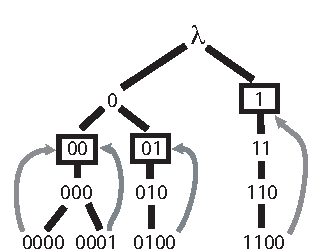
\includegraphics{pics/exthash-tree}
\caption{Reprezentace množiny $S$. Vrchol reprezentující prefix $0$, by ve
svém podstromě měl 3 prvky, což je více, než požadujeme pomocí hodnoty
$b$.}
\label{fig.hash.extern}
\end{figure}

Z obr. \ref{fig.hash.extern} plyne, že hodnota $d(S) = 2$.
\end{priklad}

\begin{tvrzeni}
Platí: Když $d(s) = k$ a prvek $t$ má stejný prefix délky $k$ jako $s$, 
pak $d(s) = d(t)$. 
\end{tvrzeni}

Reprezentace: 
\begin{itemize}
\item adresář: ke každému slovu $\alpha$ délky $d(S)$ je přiřazena adresa 
stránky, která obsahuje prvky $s \in S$, že $h(s)$ má prefix $\alpha$.
Tato slova délky $d(s)$ jsou lexikograficky uspořádána.
\item datová část: stránky s přiřazenými prvky
\end{itemize}

\begin{priklad}
Příklad adresáře pro množinu $\{0000, 0001, 0100, 1001 \}$:

\vspace{5mm}

\begin{tabular}{lll}
00 & $\rightarrow$ & 0000, 0001 \\
01 & $\rightarrow$ & 0100 \\
\hline
10 & $\searrow$ & \\
11 & $\rightarrow$ & 1001 \\
\end{tabular}
\end{priklad}

\begin{pozn}
Upřesnění reprezentace stránky (stránek): \\
Prvek $s \in S$ je uložen na stránce, která obsahuje všechny prvky $t \in
S$ takové, že prefix $h(t)$ délky $d(s)$ bude je stejný jako $h(s)$, tato stánka
bude přiřazena všem slovům $\alpha$ délky $d(S)$ takovým, že prefix $h(s)$ délky
$d(s)$ je prefix $\alpha$. \\
Pokud $\alpha$ neobsahuje žádný takový prefix, tak je mu přiřazena stránka
NIL.
\end{pozn}

\subsection{Operace ACCESS}

viz algoritmus \ref{alg:exthash.access}

\begin{algorithm}[!htb]
\caption{ACCESS pro externí hašování}
\label{alg:exthash.access}
ACCESS(x)
\begin{enumerate}
\item Spočítáme $h(x)$, natáhneme adresář, nalezneme $d(S)$ a najdeme
stránky odpovídající prefixu $h(x)$ délky $d(S)$
\item Natáhneme odpovídající stránku do paměti, zjistíme, zda obsahuje $x$ a
když ano, provedeme požadovené úpravy.
\item Stránku uložíme zpět na stejné místo.
\end{enumerate}
\end{algorithm}

Operace ACCESS vyžaduje 3 přístupy na externí medium. (za předpokladu, že
adresář je také uložen na externím mediu a zabírá jednu stránku) 

Pro rychlou implementaci aktualizačních operací je vhodné mít u každé
stránky uloženo informaci kolik je prvků na stránce.


\subsection{Operace INSERT}

viz algoritmus \ref{alg:exthash.insert}

% pozn: \mnote nesmi byt uvnitr prostredi algorithm
\begin{algorithm}[!htb]
\caption{INSERT pro externí hašování}
\label{alg:exthash.insert}
INSERT(x)
\begin{enumerate}
\item Spočítáme $h(x)$, natáhneme adresář, nalezneme $d(S)$ a nalezneme adresu
stránky odpovídající prefixu $h(x)$ délky $d(S)$. (XXX odkud vezmu $d(S)$ ?)
% XXX \mnote{$d(S)$ vezmu odkud ?}
\item Natáhneme do paměti odpovídající stránku. když v ní existuje $x$ 
$\rightarrow$ konec
\item Když neobsahuje $x$ a má méně prvků než $b$, vložíme $x$ do této stránky
a uložíme ji zpátky na stejné místo a aktualizujeme adresář (počty prvků
na stránce)
\item Když stránka prvek $x$ neobsahuje a má $b$ prvků, stránku rozdělíme
(nalezneme nové $d(s)$ pro $s$ z této stránky i s přidaným $x$), stránky 
uložíme a aktualizujeme adresář.
\end{enumerate}
\end{algorithm}
\mnote{pokud je nově nalezené $d(s) \leq d(S)$, adresář se zvětšovat nebude}

Operace INSERT vyžaduje 6 přístupů na externí medium.

\begin{pozn}
Rozštěpení stránky nemusí nutně znamenat zvětšení adresáře.
\end{pozn}

\begin{priklad}
\label{priklad:exthash.insert2}
Do množiny z příkladu \ref{priklad:exthash.tree} vložíme pomocí operace
INSERT prvek 1111. Hodnota $d(1100) = 1$ se po vložení prvku 1111
nezmění. Podstrom reprezentující prvky množiny $S$ s prefixem 11
bude mít po vložení prvku 1111 dva syny. (viz obr.
\ref{fig.hash.extern.ins})

\begin{figure}[!htb]
\centering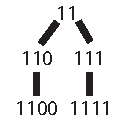
\includegraphics{pics/exthash-ins}
\caption{Podstrom reprezentující prvky množiny $S$ s prefixem 11 po
vložení prvku 1111}
\label{fig.hash.extern.ins}
\end{figure}

Pokud vezmeme situaci danou po vložení prvku 1111, bude adresář vypadat
takto:

\vspace{5mm}

\begin{tabular}{lll}
00 & $\rightarrow$ & 0000, 0001 \\
\hline
01 & $\rightarrow$ & 0100 \\
\hline
10 & $\searrow$ & 	 \\
  & &  1001 \\
11 & $\nearrow$	& \\
\end{tabular}

\vspace{5mm}

Nyní vložíme prvek 0010. V tomto případě dojde ke zvětšení adresáře:

\vspace{5mm}

\begin{tabular}{lll}
000 & $\rightarrow$ & 0000, 0001 \\
\hline
001 & $\rightarrow$ & 0010 \\
\hline
010 & $\rightarrow$ & 0100 \\
011 & $\nearrow$ & \\
\hline
100 & $\searrow$ & \\
101 & $\rightarrow$ &  1001, 1111 \\
110 & $\nearrow$ & \\
111 & $\nearrow$ & \\
\end{tabular}

\vspace{5mm}

Hodnota $d(S)$ je nyní 3.
\end{priklad}


\subsection{Operace DELETE}

viz algoritmus \ref{alg:exthash.delete}

\begin{algorithm}[!htb]
\caption{DELETE pro externí hašování}
\label{alg:exthash.delete}
DELETE(x)
\begin{enumerate}
\item spočítáme $h(x)$, natáhneme adresář, nalezneme $d(S)$, nalezneme adresu
stránky odpovídající prefixu $h(x)$ délky $d(S)$, zjistíme zda po odebrání
prvku $x$ může nastat spojování stránek a pokud ano, nalezneme adresu
stránky, která se spojí s naší stránkou
\item natáhneme odpovídající stránku do paměti, zjistíme zda obsahuje $x$,
pokud ne, tak konec
\item když obsahuje $x$ a nemůže dojít ke sloučení stránek, tak odstraníme
$x$, stránku uložíme na stejné místo a aktualizujeme adresář (počty prvků na
stránce)
\item když obsahuje a dojde ke slučování, pak odstraníme $x$, natáhneme
druhou stránku a stránky sloučíme, uložíme novou stránku a aktualizujeme
adresář.
\end{enumerate}
\end{algorithm}
\mnote{pro aktualizaci adresáře to mohou být 2 operace - načtení a
uložení. zřejmě proto, aby mohlo být současně puštěno víc operací.}

\begin{priklad}
Pro situaci z příkladu \ref{priklad:exthash.insert2} provedeme
DELETE(0100). V adresáři budou pak položky 010 a 011 ukazovat na prázdnou
stránku (NIL). Adresář zůstal po této operaci stejný.

Nyní smažeme prvek 0001.

\begin{figure}[!htb]
\centering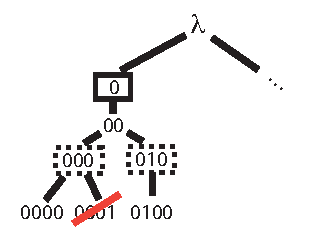
\includegraphics{pics/exthash-del}
\caption{Část stromu reprezentujícího množinu $S$ před smazáním prvku 0001}
\label{fig.hash.extern.del}
\end{figure}

Na obr. \ref{fig.hash.extern.del} je vidět, že po smazání prvku 
0001 může být adresář opět zmenšen.

Po provedení DELETE(0001) bude adresář vypadat takto:

\vspace{5mm}

\begin{tabular}{lll}
000 & $\rightarrow$ & 0000, 0010 \\
001 & $\nearrow$ & \\
\hline
010 & $\rightarrow$ & NIL \\
011 & $\nearrow$ & \\
\hline
100 & $\searrow$ & \\
101 & $\rightarrow$ &  1001, 1111 \\
110 & $\nearrow$ & \\
111 & $\nearrow$ & \\
\end{tabular}

\vspace{5mm}

Nyní můžeme provést zmenšení adresáře na:

\vspace{5mm}

\begin{tabular}{lll}
00 & $\rightarrow$ & 0000, 0010 \\
01 & $\nearrow$ & \\
\hline
10 & $\rightarrow$ & 1100, 1111	 \\
11 & $\nearrow$	& \\
\end{tabular}

\vspace{5mm}

Tento adresář můžeme ještě zmenšit:

\vspace{5mm}

\begin{tabular}{lll}
0 & $\rightarrow$ & 0000, 0010 \\
\hline
1 & $\rightarrow$ & 1100, 1111 \\
\end{tabular}
\end{priklad}

\begin{pozn}
Pesimistický odhad pro operaci DELETE je nejvýše 6 přístupů na externí 
medium.
\end{pozn}

\subsubsection{Aktualizace adresáře}

V posledním kroku DELETE se provádí aktualizace adresáře. 
Nejprve provedeme opravení odkazů na stránky: pokud u sudého záznamu v
adresáři dojde k vyprázdnění stránky, bude tam odkaz na NIL. pokud dojde k
vyprázdnění u liché stránky, přehodí se odkaz na předchozí (sudou)
stránku.

Potom se testuje, zda jde adresář zmenšit. Zmenšování provádíme tak
dlouho, dokud to jde.

\subsection{Reprezentace adresáře}

\begin{itemize}
\item reprezentovat jako posloupnost dvojic (adresa stránky, počet prvků na
stránce), kde $i$-tá dvojice je přiřazení $i$-tému slovu v lexikografickém
uspořádání.
\item zvětšování adresáře znamená zdvojení prvků
\item test na zmenšování adresáře - testujeme, zda adresa na lichém místě
je stejná jako adresa na následujícím sudém místě - pokud ano, tak zmenším
adresář vymazáním sudých členů posloupnosti.
\end{itemize}

Očekávané zaplnění stránky při rovnoměrném rozložení dat je 
$b \ln 2 \approx 0.69 b$

Očekávaná velikost adresáře je $\frac{e}{b \ln 2} n^{1 + \frac{1}{b}}$ (při
rovnoměrném rozložení dat)

\begin{pozn}
Člen $n^{1 + \frac{1}{b}}$ není lineární, zde je problém, proto se to
nehodí pro malá $b$.
\end{pozn}

\begin{tabular}{|l||l|l|l|l|}
\hline
b/n   	&$10^5$   &$10^6$ 	&$10^8$ 	&$10^{10}$    \\
\hline
2  	&$6.2*10^7$  &$1.96*10^8$	&$1.96*10^{11}$	&$1.96*10^{14}$ \\
10	&$1.2*10^5$  &$1.5*10^6$	&$2.4*10^8$	&$3.9*10^{10}$  \\
50	&$9.8*10^3$  &$1.0*10^6$	&$1.1*10^8$	&$1.2*10^{10}$  \\
100	&$4.4*10^3$  &$4.5*10^4$	&$4.7*10^6$	&$4.9*10^8$   \\
\hline
\end{tabular}

\vspace{5mm}

Jak je vidět, pro $b = 2$ se to nehodí, adresář je větší než velikost dat.

\begin{pozn}
Když pracujeme s velikostí $S$ kolem $10^{10}$, pak je vhodné, aby 
$b \geq 100$. Pro větší množiny $S$ musí být $b$ větší.
\end{pozn}

% --------------------------------------------------------------------------
\section{Perfektní hašování}

Perfektním hašováním myslíme úlohu nalézt pro danou pevnou množinu 
$S \subseteq U, |S| = n$ perfektní hašovací funkci, tj. funkci, která nemá na 
množině $S$ kolize. Tato úloha nepřipouští přirozenou implementaci 
operace INSERT, protože přidaný prvek může způsobit kolizi. 
Typický příklad použití je tabulka klíčových slov kompilátoru.

\begin{defn}
Funkce $h: U \to \intrange{0}{m-1}$ je perfektní pro $S$, když je na S
prostá ($\forall x\neq y \in S$ platí $h(x) \neq h(y)$).
\end{defn}

Za jakých podmínek lze povolit INSERT? Musí být málo
pravděpodobný. Prvky navíc se dávají jinam a po jisté době se vše
přepočítá do jedné tabulky pro novou perfektní hašovací funkci.

\begin{samepage}
Požadavky na hledanou hašovací funkci:
\begin{enumerate}
  \item $h$ je perfektní na $S$
  \item $\forall x$ je $h(x)$ rychle spočitatelná
  \item $m$ řádově srovnatelné s $n$
  \item zakódování $h$ vyžaduje málo prostoru
\end{enumerate}
\end{samepage}

Požadavky 2) a 3) jdou proti sobě. A až se nám je podaří skloubit,
budeme mít problémy s 4). A navíc hledání $h$ potrvá dlouho.

% ..........................................................................
\subsection{Perfektní hašovací funkce do tabulky velikosti $n^2$}

Využijeme, co už víme o univerzálním hašování. Pro $k \in \intrange{1}{N-1}$ 
a pro pevné $m$ definujme 
\begin{equation}
h_k(x) = ( kx \bmod N ) \bmod m, \quad\text{kde $N=|U|$ je prvočíslo.}
\end{equation}
Budeme hledat vhodná $k$, $m$.
Definujme míru perfektnosti
\begin{equation}
d = \sum_{k=1}^{N-1} \sum_{x \neq y \in S} \delta_{h_k}(x,y)
\end{equation}
a pro $k \in \intrange{1}{N-1}$ položme
\begin{equation}
b_k(i) = |\{ x \in S : h_k(x) = i \}|
\end{equation}

Jednak platí
\begin{align}
\label{bki2}
% vnitrni suma (s mocninou) dana do zavorky aby byly v poradku priority 
% (from V. Havranek)
d & = \sum_{k=1}^{N-1} \left( ( \sum_{i=0}^{m-1} ( b_k(i) )^2 ) -n \right)\\
\intertext{a také}
d & = \sum_{x \neq y \in S} |\{ k : h_k(x)=h_k(y) \}|
	&&\text{prohozením sum}\\
\end{align}

Co znamená $h_k(x) = h_k(y)$ pro $x \neq y$? Následující tvrzení jsou
ekvivalentní:
\begin{align*}
kx \bmod N & = ky \bmod N && \pmod m\\
k(x-y) \bmod N & = 0 && \pmod m\\
k(x-y) \bmod N & = r m && \text{pro } r \in 
% *ceil -> *floor (fakticka poznamka od Ladislava Proska
	\{ - \lfloor N/m \rfloor .. \lfloor N/m \rfloor \} - \{0\}, \\
\end{align*}
tedy
\[
d \leq \sum_{x \neq y \in S} 2 \frac Nm = \frac{2 n(n-1) N}m
\]
a dosazením do \eqref{bki2}, podle přihrádkového principu
\begin{equation}
\label{existsk}
\exists k : \sum_{i=0}^{m-1} ( b_k(i) )^2 \leq n + \frac{2 n(n-1)}m
\end{equation}

Pro speciální velikosti tabulky dostáváme dosazením do \eqref{existsk}:
\begin{align}
\label{3n}
&\text{Pro } m = n: 
&& \exists k \text{ nalezitelné v čase }O(nN): 
\sum_{i=0}^{m-1} ( b_k(i) )^2 < 3n\\
\label{perf}
&\text{Pro } m = 1 + n(n-1): 
&& \exists k \text{ nalezitelné v čase }O(nN):  
h_k \text{ je perfektní} 
\end{align}

\begin{proof}
Probíráme všechny možnosti pro $k$, těch je $O(N)$.
\begin{enumerate}
\item[\eqref{3n}]
Pro dané $k$ spočítáme $\sum ( b_k(i) )^2$ v čase $O(n) = O(m)$.
\item[\eqref{perf}]
$\sum ( b_k(i) )^2 \leq n + \frac{2 n(n-1)}{1+ n(n-1)} < n + 2$.
Kdyby $h_k$ nebyla perfektní, pak 
$\exists j : b_k(j) \geq 2$
a
$\sum ( b_k(i) )^2 \geq (n-2) 1^2 + 1 \cdot 2^2 = n + 2$,
spor.
Při hledání $k$ ověříme perfektnost $h_k$ v čase $O(n)$.
% zmatek s indexy u k (T. Matousek):
% Tohle by melo byt vporadku. k je jako scitaci index jen v (4.8) a (4.10)
% a dal uz ne.
% Ten soucet v d jde pres vsechny hashovaci funkce a jedna z nich je ta
% prava. Ja bych to tak nechal, je to ok. Staci smazat tu *.
\end{enumerate}
\end{proof}

Nyní máme perfektní hašovací funkci, která ale porušuje požadavek (3).
% ..........................................................................
\subsection{Perfektní hašovací funkce do tabulky velikosti $3n$}

Zkombinujeme oba výsledky z předchozí části.
% --- nejprve první funkcí hašujeme do tabulky velikosti $< 3n$

Podle \eqref{3n} nalezneme $k$ takové, že
$\sum ( b_k(i) )^2 < 3n$.

Pro každé $i \in \intrange{0}{n-1}$ vezmeme množinu kolidujících prvků
$S_i = \{ s \in S : h_k(s) = i \}$.
Označme $n_i = |S_i|$.

Podle \eqref{perf} pro každé $i$ nalezneme $k_i$ takové, že
pro $m_i = 1 + n_i(n_i-1)$ je $h_{k_i}$ perfektní pro $S_i$.

Každou zahašovanou množinu $S_i$ uložíme ve výsledné tabulce od pozice
$d_i$: 
\[
d_i = \sum_{j=0}^{i-1}(1 + n_j(n_j-1)).
\]

Konečně definujme
\[
g(x) = d_i + h_{k_i}(x),\quad\text{kde } i = h_k(x),
\]
která je perfektní a velikost tabulky je
\[
m = d_n = \sum_{j=0}^{n-1}(1 + n_j(n_j-1))
\leq \sum_{j=0}^{n-1} n_j^2
=  \sum_{j=0}^{n-1} (b_k(j))^2
< 3n
\]

Ovšem na zakódování této funkce potřebujeme hodně paměti: 
nevadí nám $d_i$, 
ale $k$ a každé $k_i$ je velikosti $O(N)$, 
tedy potřebujeme $n \log_2 N$ bitů, což odporuje našemu požadavku (4).
V dalších krocích budeme zmenšovat čísla definující hašovací funkci.
% ..........................................................................
\subsubsection{Podobná funkce daná číslem velikosti $O(N)$}

\mnote{lepší jména proměnných!}
Zvolme prvočíslo $p_1$ takové, že 
$1 +n(n-1) \leq p_1 \leq 1+ 2n(n-1)$. Nějaké takové musí existovat
(Bertrandův postulát: $\forall n>1 \exists$ provčíslo p, že 
$n < p < 2n$).
Podle \eqref{perf} %TODO, musíme dokázat m \geq, což mírně zatemní dk.
$\exists k : h_k(x) = ( kx \bmod N) \bmod p_1$ 
je perfektní na $S$.

Vytvořme
\[
S_1 = \{ h_k(s) : s \in S\} \subset \intrange{0}{p_1 -1}
\]
a na $S_1$ aplikujme předchozí sekci, kde $N = p_1$.

Dostáváme hašovací funkci $g_1$, která
\begin{itemize}
\item je perfektní pro $S$
\item je spočitatelná v čase $O(1)$ 
\item hašuje do tabulky $<3n$ 
\item je určena 1 číslem velikosti $O(N)$ \\
 \quad a $O(n)$ čísly velikosti $O(n^2)$ 
\end{itemize}

% ..........................................................................
\subsubsection{Podobná funkce daná číslem velikosti $O(n^2\log N)$}
Pro extrémní případy typu $N = 2^{10^6}$ ještě postup vylepšíme,
čímž zmenšíme velikost čísel kódujících perfektní hašovací funkci 
na $O(\log N)$.

\begin{lemma}
\label{n2logN}
Pro každou množinu $S \subseteq \intrange{0}{N-1}$ velikosti $n$ existuje
prvočíslo $p$ takové, že $f_{p}(x) = x \bmod p$ je perfektní na
$S$ a $p = O(n^2 \log N)$.
\end{lemma}

Využití: pro $S$ najdeme prvočíslo $p_0$ velikosti $O(n^2 \log N)$
takové, že $f_{p_0}$ je perfektní na $S$. Vytvoříme 
\[
S_0 = \{ f_{p_0}(s) : s \in S\} \subset \intrange{0}{p_0-1}
\]
a na $S_0$ aplikujme předchozí postup, kde $N = p_0$.

Tedy pro každou množinu $S$ velikosti $n$ existuje hašovací funkce $f$, která
\begin{itemize}
\item je perfektní pro $S$
\item je spočitatelná v čase $O(1)$ 
\item hašuje do tabulky $<3n$ 
\item je určena 2 čísly velikosti $O(n^2 \log N)$ \\
 \quad a $O(n)$ čísly velikosti $O(n^2)$ 
\end{itemize}

\begin{lemma}
\label{prvociselnidelitele}
Nechť $r$ je číslo a $p_1, \ldots, p_q$ jsou všechny jeho prvočíselné
dělitele. Pak $q=O(\log r / \log\log r)$.
\end{lemma}
\begin{proof}
\begin{align*}
r & \geq \prod_{i=1}^q p_i\\
 & > q! \\
 & = \exp(\sum_{i=1}^q \ln i) \\
 & > \exp(\int_1^q \ln x \,dx) \\
 & \geq {\left( \frac qe \right)}^q \qquad\text{kde } \exp(x)=e^x
\end{align*}
Tedy
\mnote{skok}
\[
q \leq c \frac{\ln r}{\ln\ln r} \quad\text{pro vhodnou konstantu $c$.}
\]
\end{proof}
\begin{proof}[Důkaz lemmatu \ref{n2logN}]
Předpokládejme $S = \{ x_1 < \ldots < x_n \}$.
Hašovací funkce $f_t(x) = x \bmod t$ je perfektní právě když $t$ je
nesoudělné s číslem
\[
D = \prod_{i>j} (x_i - x_j) < N^{n^2}
\]
Podle \ref{prvociselnidelitele} je mezi prvními $(c \ln D / \ln\ln D)+1$
prvočísly alespoň jedno, které nedělí $D$. Víme, že $p_k = O(k \ln
k)$, tedy 
$(c \ln D / \ln\ln D) +1$-ní prvočíslo má velikost
$O(\ln D) = O( n^2 \ln N)$.
\end{proof}
\mnote{nalezeni prvocisla $p_0$ vyzaduje cas $O(n^2\log N)$.}

% ..........................................................................
\subsection{GPERF}

Jiná konstrukce perfektní hašovací funkce je použita v programu
{\tt gperf}. Distribuován pod GPL. 
Jeho návrh je popsán v \cite{douglas-GPERF}.


% --------------------------------------------------------------------------
\def\xx{% commented out
\section{Hašování pro externí paměť}

\mnote{Tohle už Koubek nepřednáší} % - zrejme komentar od M.Vidnera
% - sice to Koubek neprednasi (prednasi se to v predmetu OZD), 
% ale u statnic se to zkousi
% Externi hashovani je popsano v jine sekci.
Adresář.

MEMBER, INSERT, DELETE

Očekávané zaplnění stránky, počet stránek, velikost adresáře --- jen
citace, tabulka pro některá čísla.
}% commented out
